\chapter[Introdução]{Introdução}
% \addcontentsline{toc}{chapter}{Introdução}

\section{Motivação}
De acordo com o Sistema de Informações sobre Mortalidade (SIM), entre 1980 e 2013, 106.093 mulheres foram vítimas de homicídio, representando em 2013 uma taxa de aproximadamente 13 homicídios femininos
diários \cite{mapa_violencia_2015}. 
No primeiro semestre de 2016 foram contabilizados 555.634 atendimentos na central de denúncias 
de violência contra a mulher, de acordo com o levantamento feito pela Secretaria de Políticas para as Mulheres (SPM). 
Aproximadamente 54\% dos atendimentos foram para prestação de informações. De acordo com \cite{portal_180}, aproximadamente 13\% dos atendimentos, são relatos de violência física (51\%), psicológica (31,1\%), moral (6,51\%), patrimonial (1,93\%), sexual (4,30\%), cárcere privado (4,86\%) e tráfico de pessoas (0,24\%).

Cenários como esse impulsionaram o governo à criação de políticas públicas (PP) 
nacionais para a redução da violência contra as mulheres, como a criação de leis (Lei Maria da Penha, Lei do Feminicídio)
e de estratégias de apoio às mulheres e de conscientização da população. Além disso, estratégias tecnológicas, como aplicativos e sites, têm sido apoiadas pelo governo e criadas pela própria população. 

Na Figura \ref{fig:sistemas_categorizados} são apresentadas algumas aplicações criadas para apoio à mulher vítima
de violência em cinco categorias: Levantamento de Dados e estatísticas, Mapeamento de riscos, Informativos, Pedido de Socorro e Apoio.

\begin{figure}[ht]
\centering
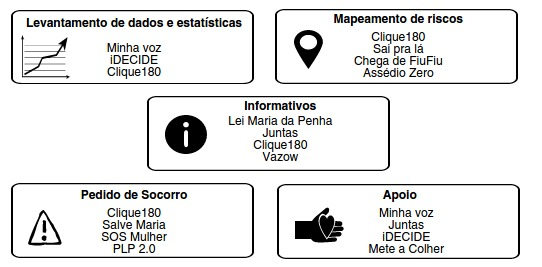
\includegraphics[scale=0.85]{figuras/sistemas_relacionados.jpeg}
\caption{Aplicações de apoio à mulher vítima de violência}
\label{fig:sistemas_categorizados}
\end{figure}

O Minha Voz foi um site criado no \textit{Hackathon} de Gênero e Cidadania da Câmara dos Deputados para apoio
às mulheres. Uma das funcionalidades é um questionário que ajuda a mulher a identificar o tipo de violência sofrida.
Já o iDECIDE, um site australiano, também conta com um questionário que apresenta para a mulher um plano de segurança 
com possíveis ações que podem ser tomadas para sair da situação de violência.

Considerando o mapeamento das aplicações, no contexto brasileiro os sistemas estão voltados para informações,
pedido de socorro e uma rede de desabafo e apoio entre as mulheres. Sendo possível perceber uma lacuna em um apoio
mais específico de acordo com a situação de violência, como sugestões de ações a serem tomadas. 

\section{Objetivo}

Considerando o contexto supracitado, o objetivo do trabalho é criar uma \textit{Application Programming Interface} (API) para uso em sistemas de tomada de decisão e planejamento de segurança para mulheres vítima de violência, através do uso de questões pré-definidas e questões inseridas pelas mulheres. 
Para esse fim os objetivos específicos do trabalho são:
\begin{itemize}
	\item Definir um questionário padrão a ser respondido pelas mulheres para apoio a tomada de decisão;
	\item Permitir que novas questões sejam inseridas pelas mulheres;
	\item Categorizar as questões (padrão e inseridas);
	\item Definir ações de segurança para as categorias de violência;
\end{itemize}






